\section{不可约分解}\label{sec:irreducible-decompositions}

上一节介绍了仿射簇不可约性的概念. 本节证明一个基本事实: 每个仿射簇都是由不可约仿射簇组成的唯一一个有限集合中各簇的并. 这是 $K[x_{1},\ldots,x_{n}]$ 是 Noether 环这一代数事实的最重要推论之一.

如果 $X$ 可约, 那么可以把 $X$ 写成仿射簇 $X_{1},X_{2}\subsetneq X$ 的并, 而 $X_{1}$ 和 $X_{2}$ 本身也可能可约. 进一步分解 $X_{1}$ 和 $X_{2}$, 就可以把 $X$ 拆成越来越多的仿射簇的并, 直到组成部分都不可约才停止. 这一过程类似于逐步把整数分解成素因数, 或把多项式分解成不可约因子. 下面的命题表明, 与整数的素因数分解或多项式的不可约分解一样, 这一过程最终会终止, 而以这种方式得到的分解是唯一的.

\begin{BookPropositionDefinition}[不可约分解]\leavevmode\label{prop:irreducible-decomposition}
  设 $X\subseteq\mathbb{A}^{n}$ 为非空仿射簇. 则存在不可约仿射簇 $X_{1},\ldots,X_{r}\subseteq X$, 使得对任意 $i\ne j$ 都有 $X_{i}\nsubseteq X_{j}$, 并且
  \begin{equation}\label{eq:irreducible-components-union}
    X=\bigcup_{i=1}^{r}X_{i}.
  \end{equation}
  此外, 除排列顺序外, 不可约仿射簇 $X_{1},\ldots,X_{r}$ 是唯一的. 我们称它们为 $X$ 的\textbf{不可约分支}, 称 \eqref{eq:irreducible-components-union} 为 $X$ 的\textbf{不可约分解}.
\end{BookPropositionDefinition}

这里应当强调, 不可约分支的数目有限, 以及对所有 $i\ne j$ 都有 $X_{i}\nsubseteq X_{j}$, 这两点对不可约分解的唯一性都至关重要. 为说明原因, 考虑抛物线 $X=\mathcal{V}(y-x^{2})\subseteq\mathbb{A}^{2}$. 因为 $X$ 已经不可约, 它的不可约分解只含一个分支. 另一方面, 若不要求 $X_{i}$ 的数目有限, 把 $X$ 写成它的所有点的并,
\[
  X=\bigcup_{p\in X}\{p\},
\]
就会得到另一个不可约分解. 如果不要求对所有 $i\ne j$ 都有 $X_{i}\nsubseteq X_{j}$, 那么也能得到不同的不可约分解, 例如
\[
  X=\{(0,0)\}\cup X.
\]

\begin{Proof}\unskip\textbf{ of Proposition~\ref{prop:irreducible-decomposition}}\quad
  我们先证明存在性, 再证明唯一性.

  (存在性) 反设 $X\subseteq\mathbb{A}^{n}$ 是一个没有有限不可约分解的非空仿射簇. 特别地, 这意味着 $X$ 不是不可约的, 所以可以写成
  \[
    X=X_{1}\cup X_{1}'\qquad\text{其中某些 }X_{1},X_{1}'\subsetneq X.
  \]
  如果 $X_{1}$ 和 $X_{1}'$ 都有有限不可约分解, 那么这两个分解的并将给出 $X$ 的一个有限不可约分解, 与假设相矛盾. 所以 $X_{1}$ 与 $X_{1}'$ 中必有一个没有有限不可约分解. 不妨设 $X_{1}$ 没有有限不可约分解, 写成
  \[
    X_{1}=X_{2}\cup X_{2}'\qquad\text{其中某些 }X_{2},X_{2}'\subsetneq X.
  \]
  同样, 因为 $X_{1}$ 没有有限不可约分解, 所以 $X_{2}$ 和 $X_{2}'$ 中至少有一个没有有限不可约分解. 假设 $X_{2}$ 没有有限不可约分解, 写成
  \[
    X_{2}=X_{3}\cup X_{3}'\qquad\text{其中某些 }X_{3},X_{3}'\subsetneq X.'
  \]
  如此继续, 就在 $\mathbb{A}^{n}$ 中构造出一条相互嵌套的无限仿射簇链:
  \[
    X\supsetneq X_{1}\supsetneq X_{2}\supsetneq X_{3}\supsetneq\cdots.
  \]
  根据 Proposition~\ref{prop:operators-reverse-inclusions}, 这给出 $K[x_{1},\ldots,x_{n}]$ 中一条相互嵌套的无限理想链:
  \[
    \mathcal{I}(X)\subsetneq\mathcal{I}(X_{1})\subsetneq\mathcal{I}(X_{2})
      \subsetneq\mathcal{I}(X_{3})\subsetneq\cdots,
  \]
  这与 $K[x_{1},\ldots,x_{n}]$ 是 Noether 环 (Corollary~\ref{cor:polynomial-rings-are-noetherian}) 矛盾. 这个矛盾蕴含每个仿射簇 $X\subseteq\mathbb{A}^{n}$ 都必定至少有一个有限不可约分解.

  (唯一性) 设
  \[
    X=\bigcup_{i=1}^{r}X_{i}=\bigcup_{j=1}^{s}Y_{j}
  \]
  是 $X$ 的两个不可约分解. 我们必须证明 $r=s$, 且必要时重新排列后, 对每个 $i$ 都有 $X_{i}=Y_{i}$. 不妨设 $r\geq s$.

  因为 $X_{1}\subseteq X$, 有
  \[
    X_{1}=X_{1}\cap X=X_{1}\cap\left(\bigcup_{j=1}^{s}Y_{j}\right)
      =\bigcup_{j=1}^{s}(X_{1}\cap Y_{j}).
  \]
  由于 $X_{1}$ 不可约, 可得对某个 $j$ 有 $X_{1}=X_{1}\cap Y_{j}$ (Exercise~\ref{ex:irreducible-variety-in-finite-union}). 重新排列 $Y_{1},\ldots,Y_{s}$, 可设 $X_{1}=X_{1}\cap Y_{1}$, 这蕴含 $X_{1}\subseteq Y_{1}$.

  同理, 由于 $Y_{1}\subseteq X$, 有
  \[
    Y_{1}=Y_{1}\cap X=Y_{1}\cap\left(\bigcup_{i=1}^{r}X_{i}\right)
      =\bigcup_{i=1}^{r}(Y_{1}\cap X_{i}),
  \]
  所以对某个 $i$ 有 $Y_{1}=Y_{1}\cap X_{i}$, 即 $Y_{1}\subseteq X_{i}$. 由此得 $X_{1}\subseteq Y_{1}\subseteq X_{i}$. 根据不可约分解的定义, 对任意 $i\ne1$ 都有 $X_{1}\nsubseteq X_{i}$, 所以必有 $i=1$. 包含关系 $X_{1}\subseteq Y_{1}\subseteq X_{1}$ 蕴含 $X_{1}=Y_{1}$.

  用 $X_{2}$ 代替 $X_{1}$ 重复这一论证, 可知对某个 $j$ 有 $X_{2}=Y_{j}$. 因为 $X_{2}\ne X_{1}$, 不可能有 $j=1$. 于是, 重新排列 $Y_{2},\ldots,Y_{s}$ 后, 可设 $X_{2}=Y_{2}$. 如此继续, 可证明对每个 $i\in\{1,\ldots,r\}$ 都有 $X_{i}=Y_{i}$. 特别地, 这证明了 $r\leq s$. 由于已经假定 $r\geq s$, 故 $r=s$, 且对所有 $i$ 都有 $X_{i}=Y_{i}$.
\end{Proof}

\begin{Example}{一个交集的不可约分支}\leavevmode\label{ex:irreducible-components-of-quadric-intersection}
  考虑仿射簇
  \[
    X=\mathcal{V}(2x^{2}+2y^{2}-z^{2}-1,x^{2}+y^{2}-1)
      \subseteq\mathbb{A}^{3}_{\mathbb{C}}.
  \]
  \BookPairedFigure
    {注意 $X=Y_{1}\cap Y_{2}$, 其中
     \[
       Y_{1}=\mathcal{V}(2x^{2}+2y^{2}-z^{2}-1)
     \]
     与
     \[
       Y_{2}=\mathcal{V}(x^{2}+y^{2}-1).
     \]
     为了对簇 $X$ 建立一些直觉, 来看 $K=\mathbb{R}$ 时的图形. 在这种情形下, $Y_{1}$ 是单叶双曲面, $Y_{2}$ 是圆柱面, 如\hyperref[fig:quadric-intersection]{右图}所示. 从图中可看出, 它们的交 $X$ 由两个圆组成.}
    {\phantomsection\label{fig:quadric-intersection}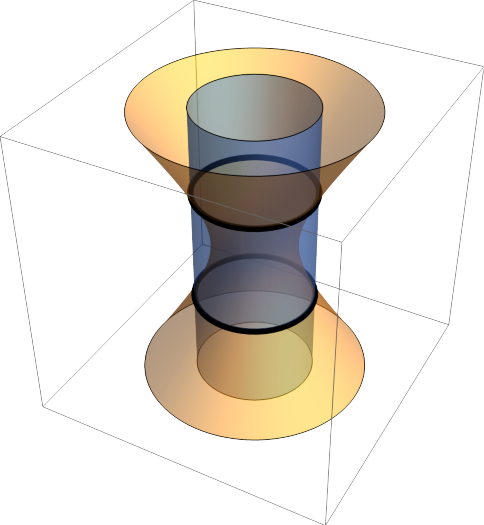
\includegraphics[width=\linewidth]{figures/quadric-intersection-two-circles.png}}
  \noindent 人们或许自然会猜测这两个圆是 $X$ 的不可约分支. 下面用代数方法验证这一直觉.

  如果 $(a,b,c)\in X$, 则其坐标满足
  \[
    2a^{2}+2b^{2}-c^{2}=1\qquad\text{且}\qquad a^{2}+b^{2}=1.
  \]
  从第一个等式中减去第二个等式的两倍, 可知这两个等式成立当且仅当
  \[
    c^{2}=1\qquad\text{且}\qquad a^{2}+b^{2}=1.
  \]
  因为 $c^{2}=1$ 当且仅当 $c=\pm1$, 所以
  \[
    \begin{aligned}
      X&=\{(a,b,1)\mid a^{2}+b^{2}=1\}\cup\{(a,b,-1)\mid a^{2}+b^{2}=1\}\\
       &=\underbrace{\mathcal{V}(x^{2}+y^{2}-1,z-1)}_{X_{1}}\cup
         \underbrace{\mathcal{V}(x^{2}+y^{2}-1,z+1)}_{X_{2}}.
    \end{aligned}
  \]
  在实数上, $X_{1}$ 和 $X_{2}$ 正是\hyperref[fig:quadric-intersection]{上图}所画的两个圆.

  为了证明 $X_{1}$ 和 $X_{2}$ 确实是 $X$ 的不可约分支, 还要证明它们各自不可约. 虽然这一事实可以在 $\mathbb{R}$ 上证明, 但在诸如 $\mathbb{C}$ 这样的代数闭域上证明要简单得多. 特别地, 在 $\mathbb{C}$ 上, 根据 Proposition~\ref{prop:vanishing-set-of-prime-ideal-is-irreducible}, 只需注意
  \[
    \langle x^{2}+y^{2}-1,z+1\rangle,\quad
    \langle x^{2}+y^{2}-1,z-1\rangle\subseteq\mathbb{C}[x,y,z]
  \]
  都是素理想. 读者不妨自行验证这一点 (见 Exercise~\ref{ex:circle-in-plane-prime-ideal}).
\end{Example}

一般而言, 判定一个簇的不可约分支并不容易, 尤其当该簇由含有许多变量的许多多项式描述, 因而无法画图来利用几何直觉时. 不过, 在簇由单个多项式 $f$ 定义的特殊情形下, $\mathcal{V}(f)$ 的不可约分解与 $f$ 的不可约分解密切相关.

\begin{Proposition}{$\mathcal{V}(f)$ 的不可约分解}\leavevmode\label{prop:hypersurface-irreducible-components}
  \strut\par\nopagebreak[4]\noindent
  如果 $f\in K[x_{1},\ldots,x_{n}]$ 的不同不可约因子为 $q_{1},\ldots,q_{m}$, 则 $\mathcal{V}(f)$ 的不可约分解为
  \[
    \mathcal{V}(f)=\mathcal{V}(q_{1})\cup\cdots\cup\mathcal{V}(q_{m}).
  \]
\end{Proposition}

\begin{Proof}
  由零点定理可知
  \[
    \mathcal{V}(f)=\mathcal{V}\bigl(\sqrt{\langle f\rangle}\bigr).
  \]
  应用 Proposition~\ref{prop:radicals-of-principal-ideals}, 可知 $\sqrt{\langle f\rangle}=\langle q_{1}\cdots q_{m}\rangle$, 所以
  \[
    \mathcal{V}(f)=\mathcal{V}(q_{1}\cdots q_{m}).
  \]
  因为 $q_{1}\cdots q_{m}$ 在某点为零当且仅当其中一个 $q_{i}$ 在该点为零, 所以
  \begin{equation}\label{eq:hypersurface-irreducible-decomposition}
    \mathcal{V}(f)=\mathcal{V}(q_{1})\cup\cdots\cup\mathcal{V}(q_{m}).
  \end{equation}
  由于每个 $q_{i}$ 都不可约, Proposition~\ref{prop:vanishing-set-of-prime-ideal-is-irreducible} 蕴含每个 $\mathcal{V}(q_{i})$ 都不可约.

  为完成证明, 必须验证对任意 $i\ne j$ 都有 $\mathcal{V}(q_{i})\nsubseteq\mathcal{V}(q_{j})$. 根据不同不可约因子的定义, 对任意 $i\ne j$ 都有 $q_{i}\nmid q_{j}$. 这蕴含对任意 $i\ne j$ 都有 $\langle q_{i}\rangle\nsupseteq\langle q_{j}\rangle$. 因为每个 $q_{i}$ 都不可约, 所以 $\langle q_{i}\rangle$ 是素理想, 而零点定理蕴含
  \[
    \mathcal{I}(\mathcal{V}(q_{i}))=\mathcal{I}(\mathcal{V}(\langle q_{i}\rangle))
      =\sqrt{\langle q_{i}\rangle}=\langle q_{i}\rangle.
  \]
  因此, 由于对任意 $i\ne j$ 都有 $\mathcal{I}(\mathcal{V}(q_{i}))\nsupseteq\mathcal{I}(\mathcal{V}(q_{j}))$, Proposition~\ref{prop:operators-reverse-inclusions} 的最后一个断言蕴含对任意 $i\ne j$ 都有 $\mathcal{V}(q_{i})\nsubseteq\mathcal{V}(q_{j})$.
\end{Proof}

\BookPairedNote
  {$K[x_{1},\ldots,x_{n}]$ 中并非每个理想都由单个多项式生成, 很自然会问, 对非主理想 $I$, 怎样计算 $\mathcal{V}(I)$ 的不可约分解? 虽然手算很困难, 但可以借助计算机完成.}
  {关于代数几何中侧重计算和算法的入门介绍, 见 Cox, Little 和 O’Shea 的书 [\ref{bib:cox-little-oshea}].}
\noindent 特别地, 给定一组生成元 $I=\langle f_{1},\ldots,f_{k}\rangle$, 有利用 Gröbner 基计算 $\mathcal{V}(I)$ 的不可约分解的有效算法. 本书选择不介绍这些计算工具, 而着重讨论代数与几何之间的词典中较偏理论的方面.

\BookExerciseHeading
\begin{BookExercises}
  \item\label{ex:irreducible-components-crossing-lines} 设 $K$ 是特征不等于 $2$ 的无限域. 证明 $\mathcal{V}(x^{2}-y^{2})\subseteq\mathbb{A}^{2}$ 的不可约分解为
    \[
      \mathcal{V}(x^{2}-y^{2})=\mathcal{V}(x+y)\cup\mathcal{V}(x-y).
    \]
    如果特征等于 $2$, 会有什么变化?
  \item\label{ex:circle-in-plane-prime-ideal} 证明
    \[
      \frac{\mathbb{C}[x,y,z]}{\langle x^{2}+y^{2}-1,z-1\rangle}
        \cong\frac{\mathbb{C}[x,y]}{\langle x^{2}+y^{2}-1\rangle}.
    \]
    据此得出 $\langle x^{2}+y^{2}-1,z-1\rangle$ 是素理想.
  \item\label{ex:quadric-intersection-real-components} 下列仿射簇的不可约分支是什么?
    \[
      \mathcal{V}(x^{2}+y^{2}+z^{2}-2z,x^{2}+y^{2}-z^{2})
        \subseteq\mathbb{A}^{3}_{\mathbb{R}}.
    \]
    (提示: 画出两个曲面, 看它们怎样相交.)
  \item\label{ex:quadric-intersection-complex-components} 求下列仿射簇的不可约分解:
    \[
      \mathcal{V}(x^{2}+y^{2}+z^{2}-2z,x^{2}+y^{2}-z^{2})
        \subseteq\mathbb{A}^{3}_{\mathbb{C}}.
    \]
    (提示: 有三个不可约分支. 复数情形的图像与上一道习题的实数情形有何不同?)
  \item\label{ex:polynomial-curve-two-irreducible-components} 求下列仿射簇的不可约分解:
    \[
      \mathcal{V}(xy+z,x^{2}-x+y^{2}+yz)\subseteq\mathbb{A}^{3}_{\mathbb{C}}.
    \]
    (提示: 有两个不可约分支.)
\end{BookExercises}
